\documentclass[10pt,a4paper]{article}

% =========================================================================
% Packages
% =========================================================================
\usepackage{iftex}
\ifxetex
  \usepackage{fontspec}
  % Menggunakan font Twentieth Century yang terinstall di sistem Windows
  \IfFontExistsTF{Twentieth Century}{
    \setmainfont{Twentieth Century}[
      AutoFakeBold=2.2,
      AutoFakeSlant=0.2,
      BoldFont={Twentieth Century},
      ItalicFont={Twentieth Century},
      BoldItalicFont={Twentieth Century}
    ]
    \newfontfamily\titlefont{Twentieth Century}[
      AutoFakeBold=3.2
    ]
  }{
    \setmainfont{Twentieth-Century.ttf}[
      Path=File/Font/,
      AutoFakeBold=2.2,
      AutoFakeSlant=0.2,
      BoldFont=Twentieth-Century.ttf,
      ItalicFont=Twentieth-Century.ttf,
      BoldItalicFont=Twentieth-Century.ttf
    ]
    \newfontfamily\titlefont{Twentieth-Century.ttf}[
      Path=File/Font/,
      AutoFakeBold=3.2
    ]
  }
\else
  \usepackage[utf8]{inputenc}
  \usepackage[T1]{fontenc}
  \usepackage[scaled=0.92]{helvet}
  \renewcommand{\familydefault}{\sfdefault}
  \providecommand{\titlefont}{}
\fi
\usepackage{geometry}
\usepackage{graphicx}
\graphicspath{{Gambar/}}
\usepackage{amsmath,amssymb}
\usepackage{xcolor}
\definecolor{headerblue}{RGB}{0, 80, 160}
\definecolor{dividerblue}{RGB}{68, 114, 196}
\usepackage{fancyhdr}
\usepackage{titlesec}
\usepackage{booktabs}
\usepackage{tabularx}
\usepackage{array}
\usepackage{caption}
\usepackage{subcaption}
\usepackage{algorithm}
\usepackage{algpseudocode}
\usepackage{hyperref}
\usepackage{microtype}
\usepackage{url}
\usepackage[nocompress]{cite}
\renewcommand\citepunct{], [}
\renewcommand\citedash{]--[}
\usepackage{float}
\usepackage{placeins}
\usepackage{enumitem}
\setlist[itemize]{label={--},leftmargin=1.5em,itemsep=1.5pt,topsep=2pt,parsep=0pt}

% =========================================================================
% Page Geometry & Margins (JTRIK Standard: A4 Paper, Margins: 2.5 cm all sides)
% =========================================================================
\geometry{
  a4paper,
  top=2.5cm,
  bottom=2.5cm,
  left=2.5cm,
  right=2.5cm,
  headheight=48pt,
  headsep=12pt,
  footskip=22pt
}

% Paragraph settings: Justified, single space, compact spacing for <= 10 pages
\setlength{\parindent}{0pt}
\setlength{\parskip}{3pt}
\linespread{1.0}

% Float Spacing Adjustments
\setlength{\floatsep}{6pt plus 2pt minus 2pt}
\setlength{\textfloatsep}{8pt plus 2pt minus 2pt}
\setlength{\intextsep}{6pt plus 2pt minus 2pt}

% Hyperlink configuration (Non-colored citations & links per JTRIK / Mendeley standard)
\hypersetup{
  hidelinks
}

% =========================================================================
% Header & Footer Settings
% =========================================================================
\pagestyle{fancy}
\fancyhf{}
\fancyhead[L]{\fontsize{8pt}{10pt}\selectfont JURNAL TEKNOLOGI REKAYASA INFORMASI DAN KOMPUTER}
\fancyfoot[R]{\fontsize{9pt}{11pt}\selectfont\thepage}
\renewcommand{\headrulewidth}{0pt}
\renewcommand{\footrulewidth}{0pt}

% First page header
\fancypagestyle{firstpage}{
  \fancyhf{}
  \fancyhead[L]{%
    \begin{minipage}[c]{0.78\textwidth}
      {\fontsize{8pt}{10pt}\selectfont JURNAL TEKNOLOGI REKAYASA INFORMASI DAN KOMPUTER}\\[1pt]
      {\fontsize{8pt}{10pt}\selectfont E-ISSN: 2797-1724, DOI: 10.000/jtrik.v1i1.2026}\\[1pt]
      {\fontsize{8pt}{10pt}\selectfont Vol. 1 No. 1 2026 pp. 01--10}
    \end{minipage}%
  }
  \fancyhead[R]{%
    \begin{minipage}[c]{0.20\textwidth}
      \raggedleft
      \IfFileExists{Gambar/image1.png}{
\includegraphics[height=1.05cm]{image1.png}}{}
    \end{minipage}%
  }
  \fancyfoot[R]{\fontsize{9pt}{11pt}\selectfont\thepage}
  \renewcommand{\headrulewidth}{1.0pt}
  \renewcommand{\headrule}{%
    \vspace{12pt}%
    {\color{dividerblue}\hrule height \headrulewidth width \headwidth}%
    \vspace{-\headrulewidth}%
  }
  \renewcommand{\footrulewidth}{0pt}
}

% =========================================================================
% Section Headings Formatting
% Level 1: 13pt Bold
% Level 2: 11pt Bold
% Level 3: 10pt Bold
% =========================================================================
\titleformat{\section}
  {\fontsize{13pt}{16pt}\bfseries}{\thesection.}{0.5em}{}
\titlespacing*{\section}{0pt}{10pt}{3pt}

\titleformat{\subsection}
  {\fontsize{11pt}{14pt}\bfseries}{\thesubsection}{0.5em}{}
\titlespacing*{\subsection}{0pt}{7pt}{2pt}

\titleformat{\subsubsection}
  {\fontsize{10pt}{12pt}\bfseries}{\thesubsubsection}{0.5em}{}
\titlespacing*{\subsubsection}{0pt}{5pt}{2pt}

% Caption styles (9 pt / small, period separator, non-bold label per JTRIK template)
\captionsetup{font={small},labelfont=normalfont,labelsep=period,justification=centering}
\captionsetup[table]{position=top,skip=3pt}
\captionsetup[figure]{position=bottom,skip=4pt}

% =========================================================================
% Document Body
% =========================================================================
\begin{document}
\thispagestyle{firstpage}

% --- Article Title (18pt Bold) ---
{\titlefont\fontsize{18pt}{22pt}\bfseries\raggedright Rancang Bangun Aplikasi Point of Sale Offline-First dengan Fitur Prediksi Penjualan Harian Menggunakan Long Short-Term Memory (LSTM)\par}
\vspace{6pt}

% --- Authors (10pt Regular) ---
{\fontsize{10pt}{12pt}\selectfont Muhammad Kholis$^{1}$, Zulfan Khairil Simbolon$^{2*}$, Azhar$^{3}$, Juneidy$^{4}$\par}
\vspace{3pt}

% --- Affiliations (8.5pt) ---
{\fontsize{8.5pt}{11pt}\selectfont
$^{1,2,3}$ Jurusan Teknologi Informasi dan Komputer, Politeknik Negeri Lhokseumawe, Jl. Banda Aceh--Medan Km. 280,3 Buketrata, Lhokseumawe 24301, Indonesia\par
$^{4}$ Program Studi Teknologi Rekayasa Multimedia Grafis, Jurusan Teknik Komputer dan Informatika, Politeknik Negeri Medan, Jl. Almamater No. 1 Kampus USU, Medan 20155, Indonesia\par}
\vspace{3pt}

% --- Corresponding Author (8.5pt) ---
{\fontsize{8.5pt}{11pt}\selectfont
*Corresponding Author: \href{mailto:zulfan@pnl.ac.id}{\underline{\textcolor{blue}{zulfan@pnl.ac.id}}}\par}
\vspace{3pt}

% --- Article Info (8.5pt) ---
{\fontsize{8.5pt}{11pt}\selectfont
\textbf{Article info:} Received August 15, 2026, Revised August 25, 2026, Accepted September 01, 2026\par}
\vspace{3pt}

% --- Open Access License (8pt) ---
{\fontsize{8pt}{10pt}\selectfont
This is an open access article under the \href{https://creativecommons.org/licenses/by-sa/4.0/}{\underline{\textcolor{blue}{CC BY-SA}}} license.\par
\vspace{2pt}
\IfFileExists{Gambar/image3.png}{
\includegraphics[height=0.70cm]{image3.png}}{%
  \IfFileExists{Gambar/template_eprotik_image1.png}{
\includegraphics[height=0.45cm]{template_eprotik_image1.png}}{}%
}\par}

\vspace{6pt}

% Divider sebelum abstrak
\vspace{1pt}
\noindent{\color{dividerblue}\rule{\textwidth}{1.5pt}}
\vspace{1pt}

% --- Abstrak (13pt Heading, 9.5pt Regular Content) ---
{\fontsize{13pt}{15pt}\bfseries Abstrak\par}
\vspace{3pt}

{\fontsize{9.5pt}{12pt}\selectfont
Usaha Mikro, Kecil, dan Menengah (UMKM) sering kali menghadapi kendala ketergantungan konektivitas internet pada sistem kasir digital serta ketidakpastian volume penjualan harian dalam perencanaan stok. Penelitian ini merancang dan membangun aplikasi \textit{Point of Sale} (POS) berbasis \textit{mobile} berarsitektur \textit{offline-first} yang mengintegrasikan fitur peramalan penjualan harian menggunakan metode \textit{Long Short-Term Memory} (LSTM), dengan studi kasus kantin EatsTEDI Sekolah Vokasi UGM. Sistem klien dikembangkan menggunakan Flutter dan basis data lokal Isar DB yang disinkronisasikan secara dua arah dengan \textit{cloud} Supabase PostgreSQL, sedangkan modul peramalan dijalankan melalui layanan REST API (Flask/TensorFlow). Pemodelan deret waktu dilakukan pada 313 data hari aktif transaksi riil menggunakan target transformasi \textit{log-return} dan dievaluasi terhadap ambang batas kelayakan operasional ($\text{sMAPE} < 20\%$). Hasil evaluasi peramalan satu langkah ke depan (\textit{one-step-ahead}) mencatat nilai rata-rata MAE sebesar Rp667.718,00, RMSE Rp897.563,00, dan sMAPE 38,06\%, yang mengindikasikan bahwa model belum memenuhi ambang batas kelayakan praktis akibat keterbatasan ukuran data (212 sekuens latih) dan tingginya variasi ritme transaksi harian. Pengujian stabilitas melalui 10 inisialisasi bobot acak (\textit{multi-seed}) menghasilkan sebaran MAE antara Rp495.527,00 hingga Rp1.048.967,00 (simpangan baku Rp145.024,00) serta rentang sMAPE 29,16\%--44,63\% (0 dari 10 \textit{seed} memenuhi ambang batas kelayakan). Kendati demikian, pengujian fungsionalitas \textit{black box} pada 12 kasus penggunaan, verifikasi sinkronisasi luring-ke-daring, serta penelusuran logika \textit{white box} pada 7 jalur kritis berhasil mencapai tingkat kesuksesan 100\% PASS, membuktikan keandalan sistem POS \textit{offline-first} dalam menjamin kelancaran transaksi kasir UMKM tanpa ketergantungan internet berkelanjutan.\par}

\vspace{4pt}
{\fontsize{9.5pt}{12pt}\selectfont\textbf{Kata Kunci:} Point of Sale, Prediksi Penjualan Harian, Long Short-Term Memory, Offline-First, Isar DB, UMKM.\par}
\vspace{6pt}
\noindent{\color{dividerblue}\rule{\textwidth}{0.8pt}}
\vspace{8pt}

% =========================================================================
% Section 1: Introduction
% =========================================================================
\section{Pendahuluan}

Sektor Usaha Mikro, Kecil, dan Menengah (UMKM) memegang peranan yang sangat penting dalam menggerakkan perekonomian nasional di Indonesia. Meskipun demikian, sebagian besar pelaku UMKM masih mengelola operasional harian secara manual atau menggunakan sistem pencatatan yang belum terintegrasi secara optimal \cite{sipayung2020}. Dalam operasional kasir (\textit{Point of Sale}/POS), banyak pelaku usaha menghadapi kendala ketergantungan konektivitas internet \cite{siddik2020}. Aplikasi kasir berbasis \textit{cloud} murni sering kali tidak dapat beroperasi ketika koneksi internet terputus, sehingga menghambat proses transaksi dan memicu antrean pelanggan. Oleh karena itu, diperlukan arsitektur sistem POS yang bersifat \textit{offline-first}, di mana transaksi kasir dapat tetap dieksekusi secara lokal dan data disinkronkan secara otomatis ketika koneksi internet kembali pulih \cite{flutter2026}.

Selain masalah keandalan transaksi di tingkat kasir, tantangan kritis lainnya yang dihadapi pemilik UMKM adalah ketidakpastian volume penjualan harian untuk pengelolaan rantai pasok dan persediaan \cite{hyndman2021}. Kurangnya estimasi permintaan yang akurat berpotensi menimbulkan kerugian finansial akibat kehabisan stok (\textit{stockout}) maupun penumpukan barang yang memicu kerusakan (\textit{overstocking}) \cite{box2015}. Peramalan deret waktu (\textit{time series forecasting}) menjadi solusi strategis dalam memproyeksikan kebutuhan operasional secara terukur \cite{hyndman2006}.

Sejumlah penelitian terdahulu telah mengkaji penerapan metode komputasi cerdas untuk peramalan penjualan ritel dengan berbagai capaian hasil. Moraes dkk. mengembangkan model hibrida CNN-LSTM bertumpuk dan paralel pada 500 deret waktu ritel selama lima tahun dengan perolehan MAPE masing-masing 14,15\% dan 14,76\% \cite{moraes2024}. Mansur dkk. mengusulkan arsitektur CNN-LSTM dengan tujuh variabel eksogen (seperti cuaca dan hari libur) pada data ritel enam bulan dan menghasilkan MAPE 4,16\%, mengungguli ANN (19,74\%) dan LSTM tunggal (10,39\%) \cite{mansur2025}. Mitra dkk. menerapkan LSTM dengan optimasi parameter hiper berbasis Keras Tuner pada dataset Walmart yang menunjukkan peningkatan akurasi signifikan dibanding metode tradisional \cite{mitra2024}. Yadav dan Barde membangun sistem prediksi penjualan waktu nyata berbasis web memadukan LSTM dan XGBoost yang terhubung ke sistem POS \cite{yadav2025}. Pada studi kasus di Indonesia, Sembiring dan Sary menguji LSTM pada kebutuhan persediaan barang dan mencatat MAPE 102--106\% dibanding Moving Average 85--88\% \cite{sembiring2025}, sedangkan Jannah dkk. membandingkan LSTM dan SARIMA pada usaha air galon \cite{jannah2025}. Selanjutnya, Verdiyanto dkk. mengembangkan aplikasi POS untuk UMKM minuman dengan Random Forest Regression \cite{verdiyanto2025}.

Meskipun model pembelajaran mendalam (\textit{deep learning}) seperti LSTM secara konseptual dirancang untuk memodelkan dependensi temporal non-linear jangka panjang \cite{hochreiter1997, goodfellow2016deep}, temuan Makridakis dkk. pada kompetisi M5 menegaskan bahwa metode statistik sederhana sering kali tetap kompetitif terhadap model jaringan saraf kompleks pada deret waktu yang pendek atau berfluktuasi tinggi \cite{makridakis2022}. Pada konteks UMKM mikro dengan data historis terbatas, model deret waktu rentan terhadap jeda kalender akademik dan ketidakstabilan inisialisasi bobot. Namun demikian, sebagian besar penelitian terdahulu belum menguji ketahanan model terhadap ambang kelayakan praktis operasional serta belum mengintegrasikan inferensi peramalan ke dalam aplikasi POS \textit{mobile offline-first}.

Berdasarkan latar belakang tersebut, penelitian ini merancang dan membangun sistem aplikasi \textit{Point of Sale} berbasis \textit{mobile} dengan arsitektur \textit{offline-first} menggunakan \textit{framework} Flutter dan Isar DB yang terhubung ke Supabase PostgreSQL, serta mengintegrasikan modul peramalan penjualan harian berbasis model LSTM yang di-\textit{deploy} sebagai REST API Flask pada Hugging Face. Penelitian ini mengevaluasi kinerja model LSTM secara mendalam melalui skema prediksi satu langkah ke depan (\textit{one-step-ahead}) serta pengujian stabilitas \textit{multi-seed} terhadap ambang batas kelayakan praktis ($\text{sMAPE} < 20\%$) menggunakan data transaksi riil kantin EatsTEDI UGM selama 313 hari aktif. Pengujian fungsionalitas sistem dilakukan secara komprehensif melalui metode \textit{black box}, pengujian sinkronisasi \textit{offline-first}, dan pengujian \textit{white box} pada jalur kode fungsi kritis.

% =========================================================================
% Section 2: Methods
% =========================================================================
\section{Metode Penelitian}

\subsection{Alur Penelitian}
Penelitian ini dilaksanakan sebagai penelitian pengembangan (\textit{Research and Development}) dengan pendekatan kuantitatif. Alur penelitian terbagi ke dalam dua fase terintegrasi: fase pengembangan sistem \textit{Point of Sale} dan fase pengembangan model prediksi penjualan deret waktu menggunakan LSTM, sebagaimana diilustrasikan pada Gambar \ref{fig:alur_penelitian}.

\begin{figure}[htbp]
  \centering
  \IfFileExists{Gambar/arsitektur_sistem_bw.png}{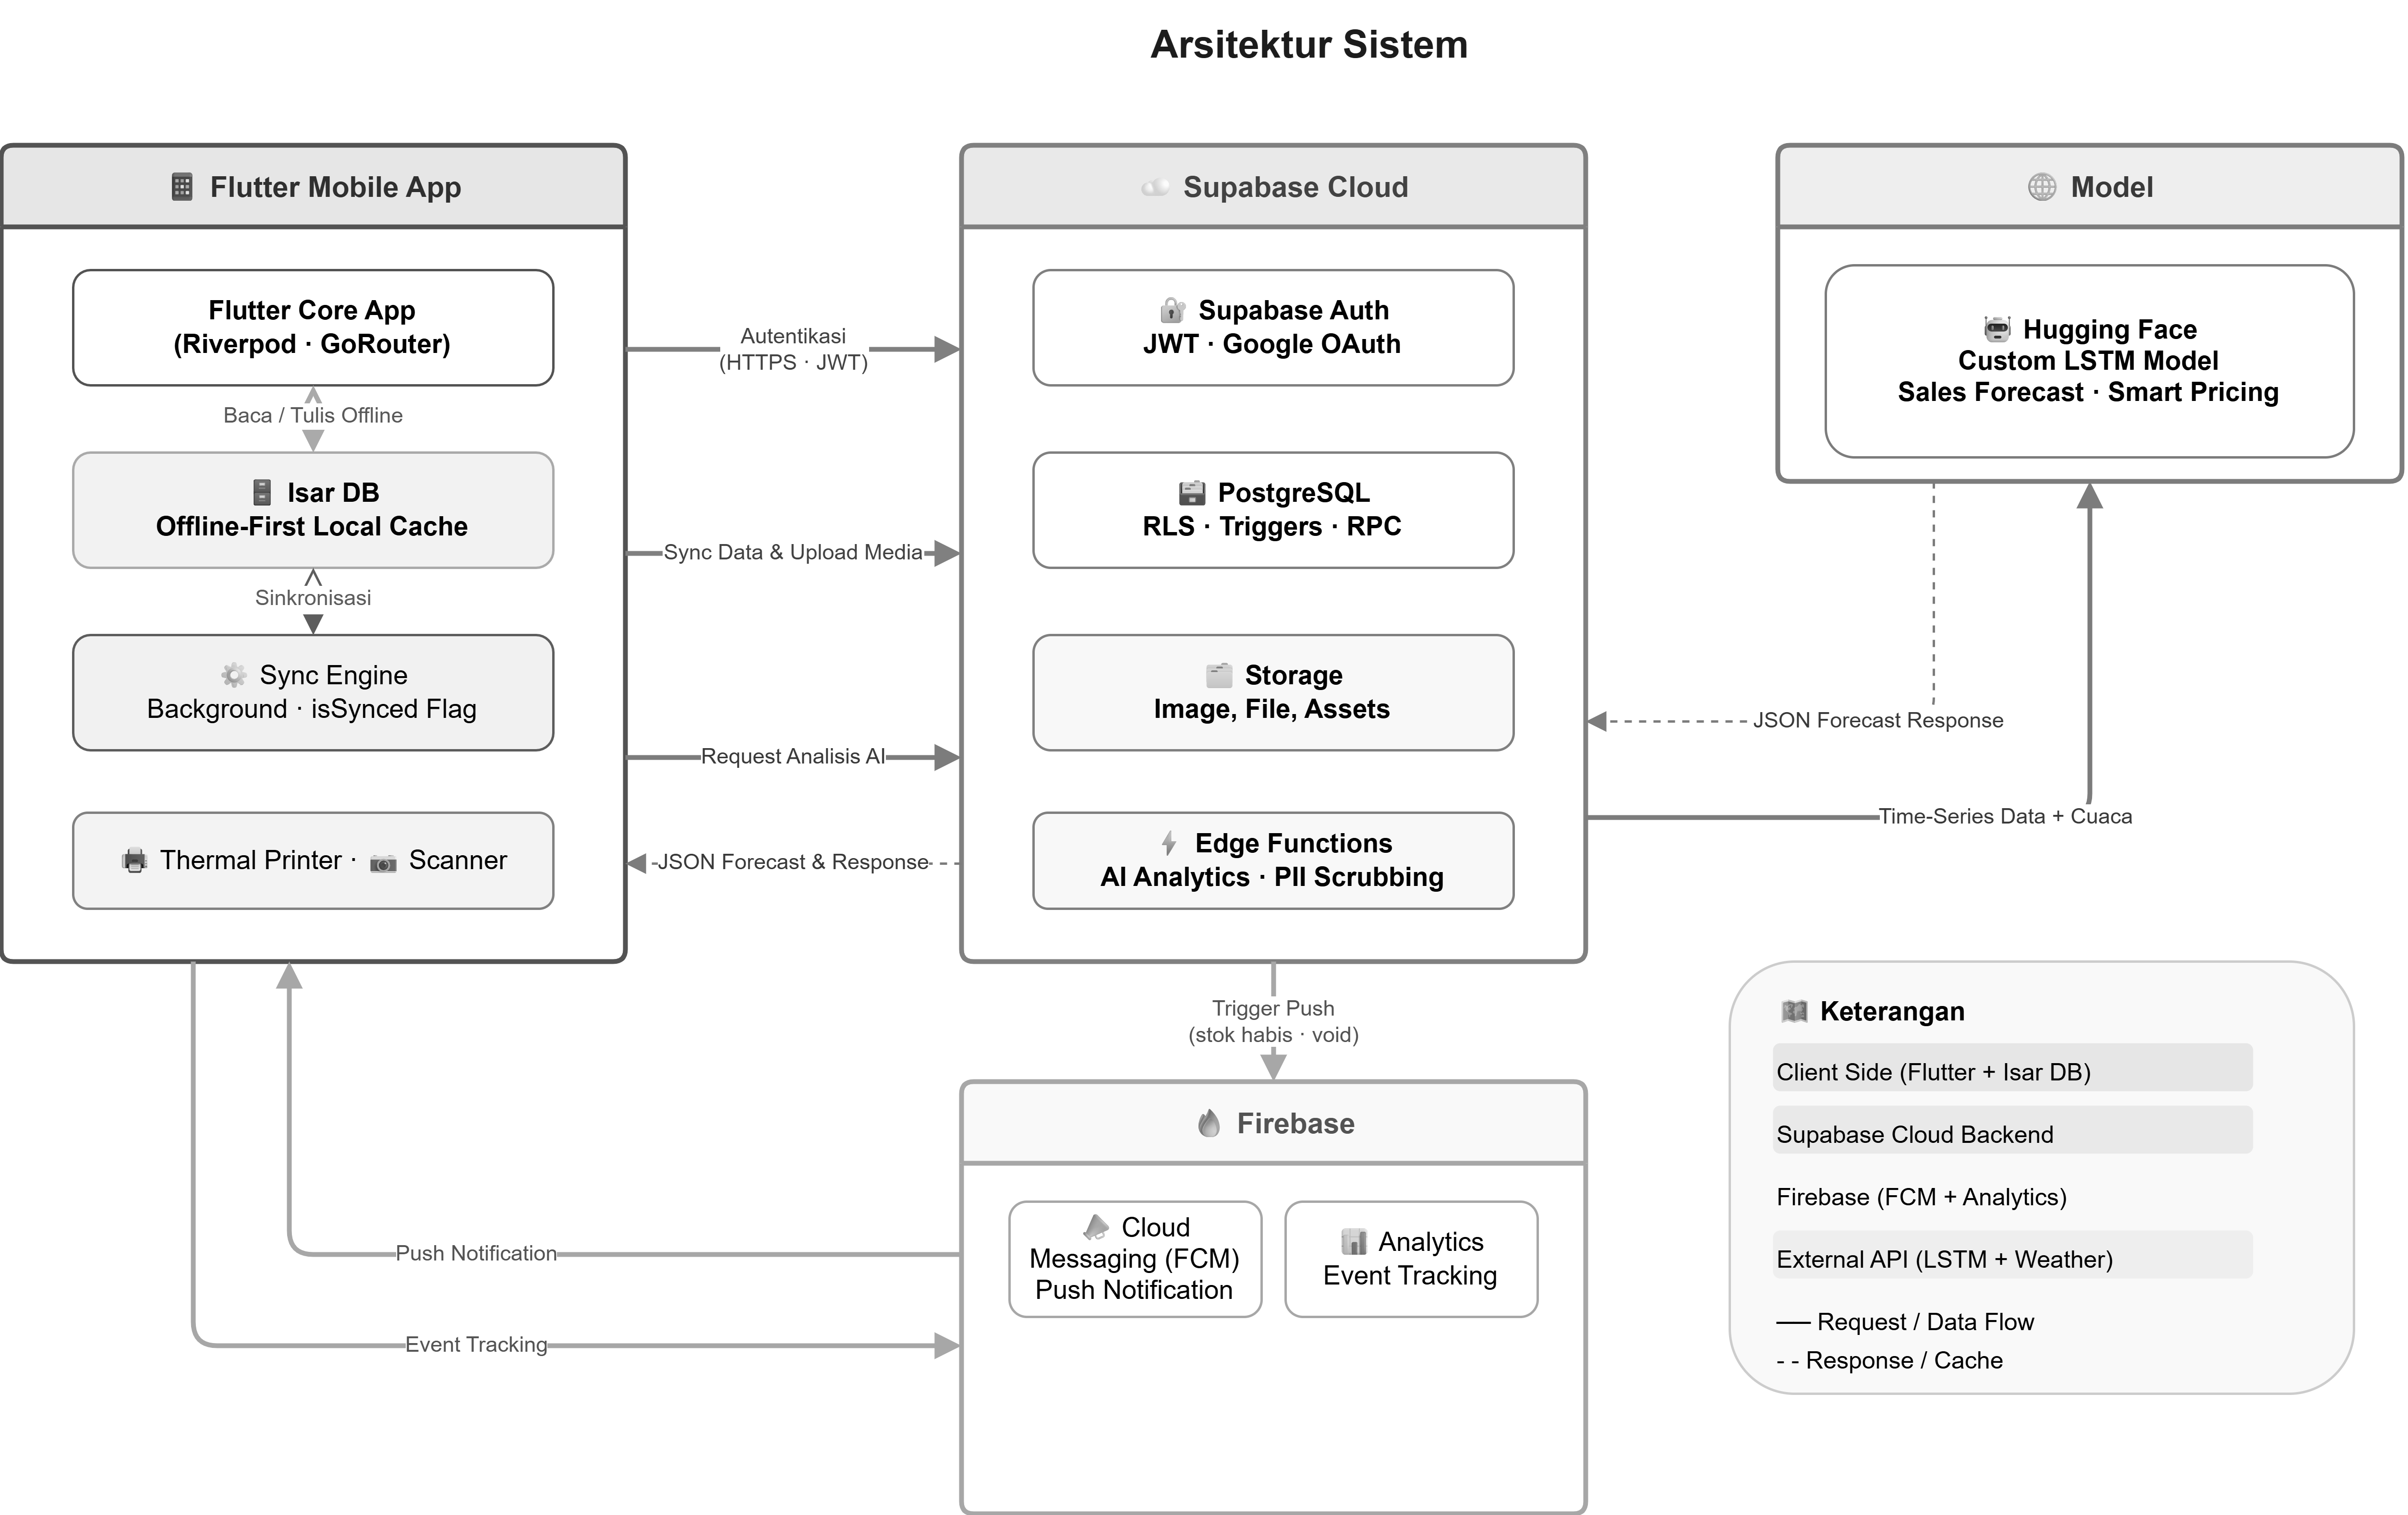
\includegraphics[width=0.75\textwidth]{arsitektur_sistem_bw.png}}{\fbox{Diagram Arsitektur Sistem POS}}
  \caption{Arsitektur Sistem POS Mobile Offline-First Terintegrasi Layanan Prediksi LSTM}
  \label{fig:alur_penelitian}
\end{figure}

\subsection{Arsitektur Sistem POS Offline-First}
Arsitektur sistem dirancang untuk menjamin kelangsungan operasional transaksi kasir tanpa ketergantungan koneksi internet secara terus-menerus. Sistem terdiri atas empat komponen utama (Gambar \ref{fig:alur_penelitian}):
\begin{itemize}
  \item Aplikasi Mobile (Sisi Klien): Dibangun menggunakan \textit{framework} Flutter (bahasa Dart) dengan arsitektur manajemen \textit{state} Riverpod \cite{flutter2026, remi2023riverpod}. Penyimpanan lokal ditangani oleh Isar Database \cite{isar2024docs} yang menyimpan data produk, kategori, dan transaksi secara instan. Komponen \textit{Sync Engine} secara berkala memeriksa status konektivitas jaringan; apabila koneksi internet terhubung, sistem mengunggah nota transaksi lokal yang memiliki status \texttt{is\_synced = false} ke basis data \textit{cloud}.
  \item Infrastruktur Cloud (Supabase): Menggunakan platform Supabase PostgreSQL sebagai basis data relasional terpusat yang dilengkapi \textit{Row Level Security} (RLS) \cite{supabase2024docs} serta prosedur tersimpan (\textit{Remote Procedure Call}/RPC) \texttt{create\_transaction\_v4} untuk memproses pencatatan transaksi dan pengurangan stok secara atomik.
  \item Layanan Telemetri dan Notifikasi (Firebase): Menggunakan Firebase Cloud Messaging (FCM) untuk pengiriman notifikasi \textit{broadcast} antarkaryawan dan peringatan stok menipis, serta Firebase Analytics untuk telemetri penggunaan fitur aplikasi.
  \item Layanan Inferensi Prediksi (Hugging Face): Model LSTM dikemas dalam layanan REST API berbasis Flask di platform Hugging Face Spaces. Aplikasi klien mengirimkan riwayat penjualan agregat melalui protokol HTTPS dan menerima hasil proyeksi penjualan dalam format JSON.
\end{itemize}

\subsection{Dataset dan Pra-pemrosesan Data Penjualan}
Dataset yang digunakan berasal dari transaksi riil kantin EatsTEDI UGM pada rentang waktu 26 Oktober 2024 hingga 4 September 2025. Dari total rentang waktu tersebut, dilakukan pra-pemrosesan data sebagai berikut:
\begin{itemize}
  \item Penyaringan Hari Aktif: Memfilter dan mempertahankan hari-hari operasional yang memiliki transaksi penjualan positif ($\text{revenue} > 0$), menghasilkan 313 hari aktif transaksi. Hari libur kalender akademik dan akhir pekan tanpa penjualan dieliminasi untuk membentuk deret waktu aktif teratur.
  \item Transformasi Target Log-Return: Untuk mengatasi ketidakstasioneran data omzet nominal yang memiliki rentang fluktuasi lebar, target model ditransformasikan ke dalam bentuk \textit{log-return} harian ($r_t$):
  \begin{equation}
    r_t = \ln\left(\frac{Y_t + 1}{Y_{t-1} + 1}\right)
    \label{eq:log_return}
  \end{equation}
  di mana $Y_t$ adalah nilai omzet penjualan nominal pada hari aktif ke-$t$. Penambahan konstanta $+1$ bertujuan mencegah timbulnya nilai tak terdefinisi saat omzet bernilai nol.
  \item Fitur Siklik Temporal: Ekstraksi fitur hari kerja berupa representasi trigonometri siklik siklus mingguan:
  \begin{equation}
    \sin_{\text{dow}} = \sin\left(\frac{2\pi \cdot d}{7}\right), \quad \cos_{\text{dow}} = \cos\left(\frac{2\pi \cdot d}{7}\right)
    \label{eq:dow}
  \end{equation}
  di mana $d \in \{0, 1, \dots, 6\}$ menyatakan indeks hari dalam sepekan.
  \item Normalisasi dan Pembentukan Sequence: Fitur numerik dinormalisasi menggunakan Min-Max Scaling ke rentang $[0, 1]$ \cite{pedregosa2011scikit}. Pembentukan sampel pembelajaran terawasi (\textit{supervised learning}) dilakukan dengan metode \textit{sliding window} berjangka pandang 7 hari aktif ($LOOK\_BACK=7$), menghasilkan dimensi masukan sekuens sebesar $7 \times 8$.
  \item Pembagian Dataset Kronologis: Dataset dibagi secara kronologis (\textit{time-based split}) dengan rasio 70\% untuk data latih (212 sampel sekuens), 15\% untuk data validasi (45 sampel sekuens), dan 15\% untuk data uji (46 sampel sekuens).
\end{itemize}

\subsection{Arsitektur Model Long Short-Term Memory (LSTM)}
Model LSTM dirancang untuk mempelajari keterkaitan temporal pada deret waktu \cite{hochreiter1997}. Perhitungan di dalam satu unit sel LSTM pada langkah waktu $t$ diatur oleh empat mekanisme gerbang (\textit{gating mechanism}):
\begin{align}
  \mathbf{f}_t &= \sigma\left(\mathbf{W}_f \cdot [\mathbf{h}_{t-1}, \mathbf{x}_t] + \mathbf{b}_f\right) \label{eq:forget_gate} \\
  \mathbf{i}_t &= \sigma\left(\mathbf{W}_i \cdot [\mathbf{h}_{t-1}, \mathbf{x}_t] + \mathbf{b}_i\right) \label{eq:input_gate} \\
  \tilde{\mathbf{C}}_t &= \tanh\left(\mathbf{W}_C \cdot [\mathbf{h}_{t-1}, \mathbf{x}_t] + \mathbf{b}_C\right) \label{eq:candidate_cell} \\
  \mathbf{C}_t &= \mathbf{f}_t \odot \mathbf{C}_{t-1} + \mathbf{i}_t \odot \tilde{\mathbf{C}}_t \label{eq:cell_update} \\
  \mathbf{o}_t &= \sigma\left(\mathbf{W}_o \cdot [\mathbf{h}_{t-1}, \mathbf{x}_t] + \mathbf{b}_o\right) \label{eq:output_gate} \\
  \mathbf{h}_t &= \mathbf{o}_t \odot \tanh(\mathbf{C}_t) \label{eq:hidden_state}
\end{align}
di mana $\mathbf{f}_t, \mathbf{i}_t, \mathbf{o}_t$ masing-masing menyatakan vektor gerbang lupa (\textit{forget gate}), gerbang masukan (\textit{input gate}), dan gerbang keluaran (\textit{output gate}); $\mathbf{C}_t$ adalah \textit{cell state}; $\mathbf{h}_t$ adalah \textit{hidden state}; $\sigma(\cdot)$ adalah fungsi aktivasi sigmoid; dan $\odot$ melambangkan perkalian elemen per elemen (\textit{Hadamard product}).

Potongan kode dan prosedur konstruksi arsitektur model LSTM Hybrid dirangkum pada Algoritma \ref{alg:lstm_model}, sedangkan rincian parameter hiper pelatihan disajikan pada Tabel \ref{tab:param_pelatihan}. Model dioptimasi dengan algoritma Adam \cite{kingma2015adam} serta menerapkan lapisan \textit{dropout} \cite{srivastava2014dropout} untuk mencegah terjadinya \textit{overfitting}.

\begin{algorithm}[htbp]
\caption{Konstruksi Model LSTM Hybrid Residual Berbasis TensorFlow/Keras}
\label{alg:lstm_model}
\fontsize{8.5pt}{10.5pt}\selectfont
\begin{algorithmic}[1]
\Require Sekuens masukan $\mathbf{X}_t \in \mathbb{R}^{7 \times 8}$ (horizon $look\_back = 7$, $n\_features = 8$).
\Ensure Estimasi nilai \textit{log-return} omzet penjualan $\hat{r}_t \in \mathbb{R}$.
\State $\text{model} \gets \text{Sequential}()$
\State $\text{model}.\text{add}(\text{LSTM}(\text{units}=24, \text{input\_shape}=(7, 8), \text{return\_sequences}=\text{False}))$
\State $\text{model}.\text{add}(\text{Dropout}(\text{rate}=0.1))$
\State $\text{model}.\text{add}(\text{Dense}(\text{units}=16, \text{activation}=\text{'relu'}))$
\State $\text{model}.\text{add}(\text{Dense}(\text{units}=1, \text{activation}=\text{'linear'}))$
\State $\text{model}.\text{compile}(\text{optimizer}=\text{Adam}(\text{lr}=5 \times 10^{-4}), \text{loss}=\text{'mse'}, \text{metrics}=[\text{'mae'}])$
\State \Return $\text{model}$
\end{algorithmic}
\end{algorithm}

\begin{table}[htbp]
  \centering
  \caption{Konfigurasi Parameter Hiper Pelatihan Model LSTM}
  \label{tab:param_pelatihan}
  \fontsize{8.5pt}{11pt}\selectfont
  \begin{tabular}{ll}
    \toprule
    \textbf{Parameter Hiper} & \textbf{Nilai / Konfigurasi} \\
    \midrule
    Dimensi Masukan & $7 \times 8$ ($LOOK\_BACK = 7$ hari aktif, 8 fitur) \\
    Lapisan Tersembunyi LSTM & 1 lapisan, 24 unit sel LSTM \\
    Tingkat Dropout & 0,1 \\
    Lapisan Fully Connected & Dense 16 neuron (aktivasi ReLU) \\
    Lapisan Output & Dense 1 neuron linier (prediksi \textit{log-return}) \\
    Total Parameter Terlatih & 3.585 parameter \\
    Optimizer & Adam ($\text{learning rate} = 5 \times 10^{-4}$) \\
    Fungsi Kerugian (\textit{Loss}) & Mean Squared Error (MSE) \\
    Ukuran Batch & 16 \\
    Maksimum Epoch & 200 (dengan Early Stopping \textit{patience} 20 \& ReduceLROnPlateau) \\
    \bottomrule
  \end{tabular}
\end{table}

\subsection{Rekonstruksi Nilai Nominal dan Proyeksi Multi-Langkah}
Nilai keluaran estimasi \textit{log-return} $\hat{r}_t$ direkonstruksi kembali ke skala nominal Rupiah ($\hat{Y}_t$) menggunakan rumus eksponensial inversi:
\begin{equation}
  \hat{Y}_t = \exp\left(\ln(Y_{t-1} + 1) + \hat{r}_t\right) - 1
  \label{eq:rekonstruksi}
\end{equation}

Untuk proyeksi multi-langkah ke depan secara rekursif hingga horizon 7 hari aktif, sistem menerapkan tiga mekanisme pengaman (\textit{safety guard}):
\begin{itemize}
  \item \textit{Clipping}: Membatasi \textit{log-return} prediksi dalam persentil 10 hingga 90 dari data latih untuk mengeliminasi lonjakan tak wajar.
  \item \textit{Damping}: Mengalikan nilai variasi perubahan dengan faktor redaman $\phi^{h-1}$ ($\phi = 0,7$) seiring bertambahnya horizon langkah $h$.
  \item \textit{Safety Rail}: Membatasi omzet nominal proyeksi agar tidak melebihi nilai batas atas omzet historis (\textit{revenue ceiling}).
\end{itemize}

\subsection{Metrik Evaluasi dan Ambang Kelayakan}
Performa akurasi peramalan diuji pada skema satu langkah ke depan (\textit{one-step-ahead}) menggunakan tiga metrik evaluasi secara simultan \cite{hyndman2006, hodson2022}:
\begin{align}
  \text{MAE} &= \frac{1}{N} \sum_{t=1}^N \left| Y_t - \hat{Y}_t \right| \label{eq:mae} \\
  \text{RMSE} &= \sqrt{\frac{1}{N} \sum_{t=1}^N \left( Y_t - \hat{Y}_t \right)^2} \label{eq:rmse} \\
  \text{sMAPE} &= \frac{100\%}{N} \sum_{t=1}^N \frac{\left| Y_t - \hat{Y}_t \right|}{\left( \left| Y_t \right| + \left| \hat{Y}_t \right| \right) / 2} \label{eq:smape}
\end{align}
di mana $Y_t$ adalah omzet penjualan aktual, $\hat{Y}_t$ adalah omzet prediksi, dan $N$ adalah jumlah sampel data uji ($N=46$). Metrik sMAPE digunakan sebagai acuan utama kelayakan praktis operasional karena bersifat simetris, bebas skala, dan tidak mengalami galat ledakan (\textit{exploding error}) pada nilai omzet kecil. Ambang batas kelayakan praktis ditetapkan pada $\text{sMAPE} < 20\%$.

% =========================================================================
% Section 3: Results and Discussion
% =========================================================================
\section{Hasil dan Pembahasan}

\subsection{Evaluasi Model Prediksi LSTM terhadap Ambang Kelayakan}
Pengujian model pada data uji (46 sampel aktif) dievaluasi dalam dua skenario pengujian yang dirancang secara ketat. Skenario pertama menguji akurasi model LSTM Hybrid pada skema satu langkah ke depan (\textit{one-step-ahead}). Hasil perbandingan antara nilai aktual dan prediksi model disajikan pada Tabel \ref{tab:skenario1}.

\begin{table}[htbp]
  \centering
  \caption{Performa Model LSTM Hybrid pada Data Uji (One-Step-Ahead)}
  \label{tab:skenario1}
  \fontsize{8.5pt}{11pt}\selectfont
  \begin{tabular}{lccc}
    \toprule
    \textbf{Model / Arsitektur} & \textbf{MAE (Rp)} & \textbf{RMSE (Rp)} & \textbf{sMAPE (\%)} \\
    \midrule
    LSTM Hybrid (Rata-rata 10 Seed) & 667.718 & 897.563 & 38,06\% \\
    \textbf{Ambang Batas Kelayakan Praktis} & -- & -- & $\mathbf{< 20,00\%}$ \\
    \bottomrule
  \end{tabular}
\end{table}

Berdasarkan Tabel \ref{tab:skenario1}, model LSTM Hybrid memperoleh nilai rata-rata MAE sebesar Rp667.718,00, RMSE sebesar Rp897.563,00, dan sMAPE sebesar 38,06\%. Nilai sMAPE tersebut melampaui ambang batas kelayakan praktis 20\% yang telah ditetapkan. Visualisasi perbandingan deret waktu antara omzet aktual dan omzet hasil prediksi disajikan pada Gambar \ref{fig:prediksi_aktual}.

\begin{figure}[htbp]
  \centering
  \IfFileExists{Gambar/prediksi_vs_aktual.png}{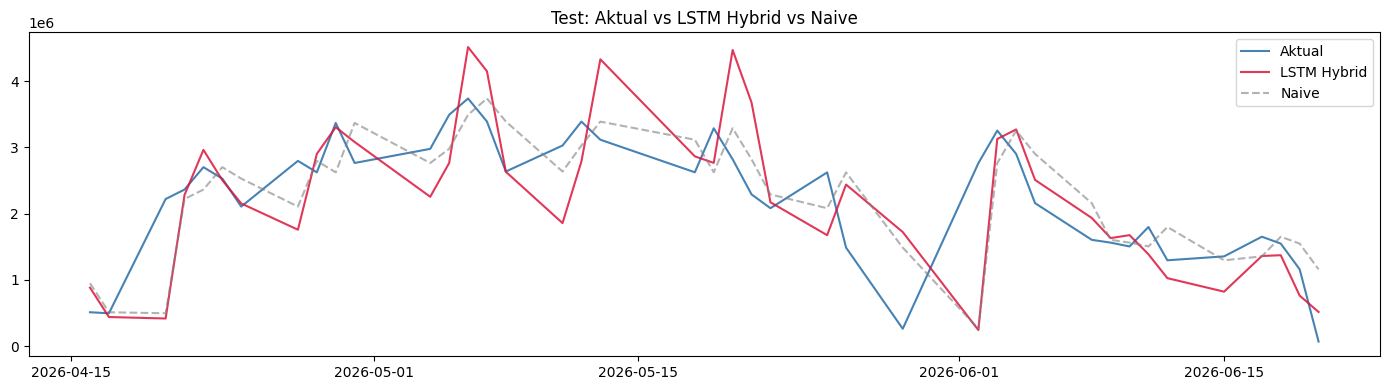
\includegraphics[width=0.75\textwidth]{prediksi_vs_aktual.png}}{\fbox{Grafik Prediksi vs Aktual}}
  \caption{Perbandingan Deret Waktu Pendapatan Aktual terhadap Prediksi Model LSTM Hybrid}
  \label{fig:prediksi_aktual}
\end{figure}

Pola grafik pada Gambar \ref{fig:prediksi_aktual} memperlihatkan bahwa model LSTM cenderung melakukan penghalusan prediksi secara berlebihan (\textit{over-smoothing}). Model mampu mengikuti tren dasar jangka menengah, namun gagal mengantisipasi lonjakan-lonjakan ekstrem omzet harian yang dipicu oleh dinamika jadwal akademik kampus dan aktivitas mahasiswa.

\subsection{Pengujian Stabilitas Model melalui Evaluasi Multi-Seed}
Skenario kedua mengevaluasi stabilitas model terhadap variasi inisialisasi bobot acak awal. Pengujian dilakukan dengan melatih ulang model sebanyak 10 kali menggunakan nilai \textit{seed} yang berbeda secara acak ($seed \in \{0, 1, \dots, 9\}$). Ringkasan statistik performa dari 10 \textit{seed} disajikan pada Tabel \ref{tab:multiseed}.

\begin{table}[htbp]
  \centering
  \caption{Statistik Performa Model LSTM Hybrid pada Pengujian Multi-Seed (10 Kali Pelatihan)}
  \label{tab:multiseed}
  \fontsize{8.5pt}{11pt}\selectfont
  \begin{tabular}{lccc}
    \toprule
    \textbf{Metrik Evaluasi} & \textbf{Rata-rata} & \textbf{Simpangan Baku ($\pm$)} & \textbf{Rentang (Min -- Maks)} \\
    \midrule
    MAE (Rp)   & 667.718 & 145.024 & 495.527 -- 1.048.967 \\
    RMSE (Rp)  & 897.563 & 165.804 & 703.721 -- 1.320.587 \\
    sMAPE (\%) & 38,06\% & 3,96\%  & 29,16\% -- 44,63\%   \\
    \bottomrule
  \end{tabular}
\end{table}

Hasil pada Tabel \ref{tab:multiseed} menunjukkan deviasi standar yang cukup tinggi, yaitu sebesar Rp145.024,00 pada MAE dan 3,96\% pada sMAPE. Nilai galat terburuk (MAE Rp1.048.967,00) tercatat lebih dari dua kali lipat galat terbaik (MAE Rp495.527,00). Dari 10 kali percobaan yang dilakukan, tidak ada satu pun \textit{seed} yang mampu mencapai nilai sMAPE di bawah ambang kelayakan 20\% (nilai terbaik berada pada \textit{seed} ke-7 dengan sMAPE 29,16\%). Sebaran distribusi nilai MAE hasil pengujian \textit{multi-seed} divisualisasikan dalam bentuk \textit{boxplot} pada Gambar \ref{fig:boxplot}.

\begin{figure}[htbp]
  \centering
  \IfFileExists{Gambar/boxplot_multiseed.png}{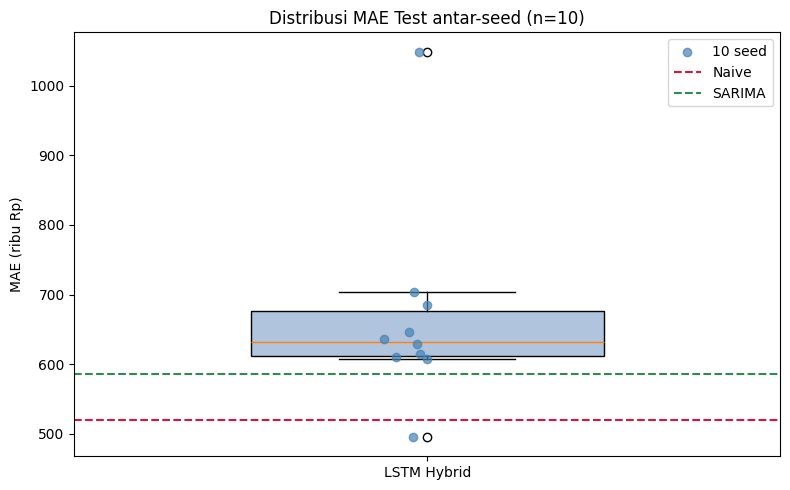
\includegraphics[width=0.48\textwidth]{boxplot_multiseed.png}}{\fbox{Boxplot Multi-Seed MAE}}
  \caption{Distribusi Sebaran MAE Model LSTM Hybrid pada Pengujian Multi-Seed (10 Pengulangan)}
  \label{fig:boxplot}
\end{figure}

Tingginya rentang sebaran ini membuktikan bahwa pelatihan jaringan saraf tiruan berulang pada ukuran data kecil (hanya 212 sekuens latih) sangat rentan terhadap variasi inisialisasi bobot acak (\textit{seed variance}). Temuan ini menegaskan bahwa pelaporan kinerja model peramalan \textit{deep learning} pada data kecil berbasis uji coba tunggal (\textit{single-run}) berisiko tinggi menyesatkan. Rekapitulasi hasil dari kedua skenario evaluasi model dirangkum pada Tabel \ref{tab:rekap_skenario}.

\begin{table}[htbp]
  \centering
  \caption{Rekapitulasi Hasil Pengujian Kedua Skenario Model Prediksi}
  \label{tab:rekap_skenario}
  \fontsize{8.5pt}{10.5pt}\selectfont
  \begin{tabularx}{\textwidth}{cp{4.2cm}cp{6.2cm}}
    \toprule
    \textbf{Skenario} & \textbf{Tujuan Pengujian} & \textbf{Ambang Terpenuhi?} & \textbf{Temuan Utama} \\
    \midrule
    1 & Mengukur akurasi satu langkah ke depan (\textit{one-step-ahead}) terhadap ambang sMAPE $< 20\%$ & Tidak & Rata-rata MAE Rp667.718,00 dan sMAPE 38,06\%, melampaui ambang batas kelayakan praktis. \\
    \midrule
    2 & Menguji kestabilan pelatihan model melalui 10 \textit{seed} acak berbeda & Tidak & Sebaran MAE sangat lebar (Rp495.527--Rp1.048.967) dengan deviasi Rp145.024; 0 dari 10 \textit{seed} memenuhi sMAPE $< 20\%$. \\
    \bottomrule
  \end{tabularx}
\end{table}

\subsection{Implementasi Antarmuka Sistem POS Mobile}
Aplikasi POS berbasis \textit{mobile} telah berhasil diimplementasikan pada perangkat Android dengan antarmuka modern yang intuitif. Sistem menyediakan fitur operasional kasir lengkap, manajemen katalog produk, mutasi stok, dasbor omzet penjualan, serta halaman analitik prediktif (\textit{Smart Analytics}) yang menyajikan proyeksi penjualan 7 hari ke depan hasil inferensi model LSTM (Gambar \ref{fig:ui_smart_analytics}).

\begin{figure}[htbp]
  \centering
  \IfFileExists{Gambar/smart_analytics.png}{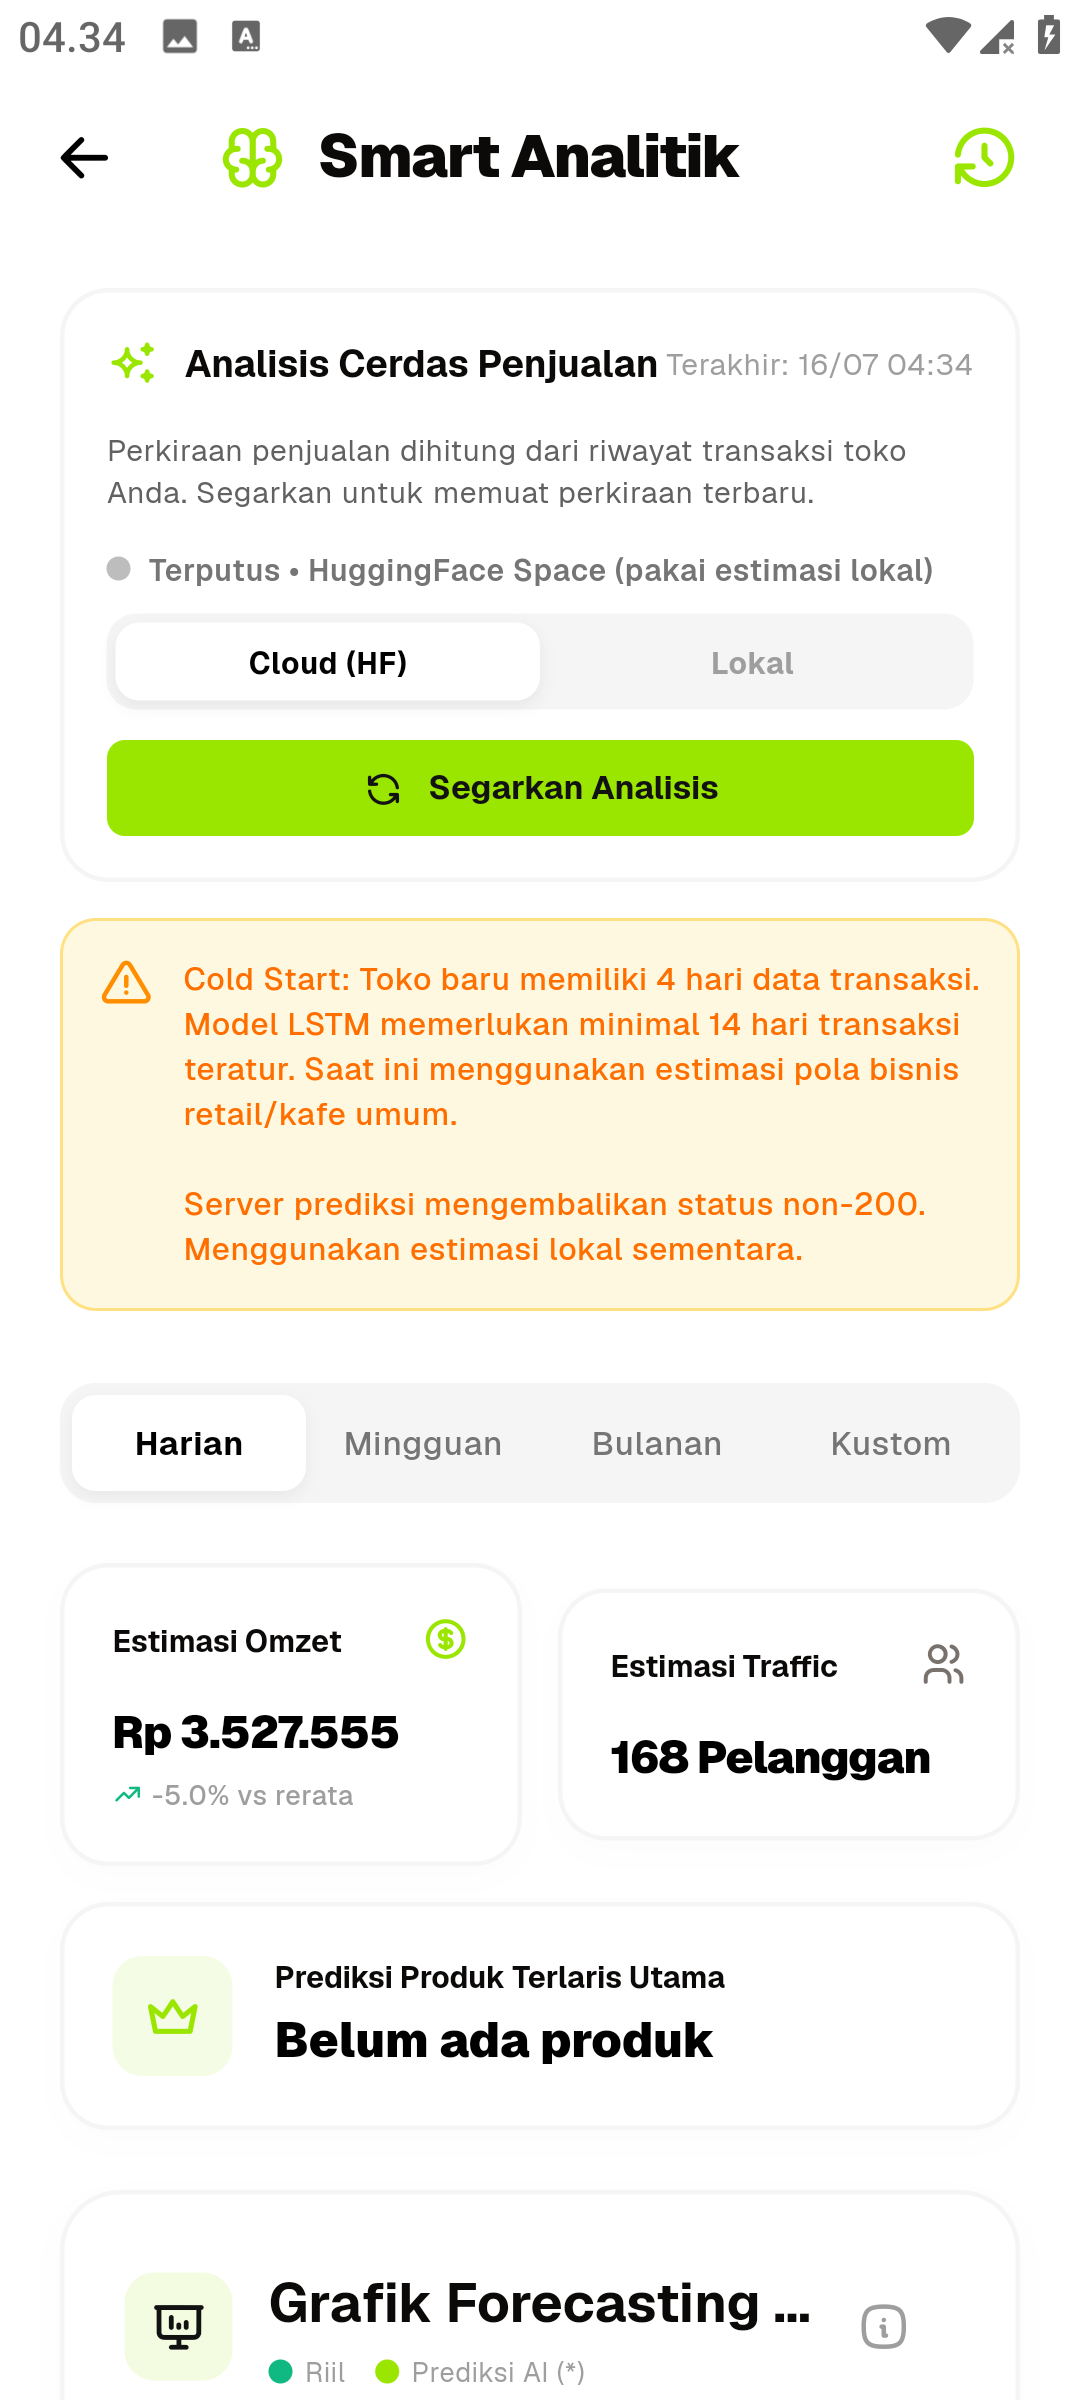
\includegraphics[width=0.45\textwidth]{smart_analytics.png}}{\fbox{Halaman Smart Analytics POS}}
  \caption{Implementasi Antarmuka Fitur Smart Analytics pada Aplikasi POS Mobile}
  \label{fig:ui_smart_analytics}
\end{figure}

Halaman \textit{Smart Analytics} menampilkan estimasi omzet, grafik proyeksi multi-langkah dengan batas atas pengaman (\textit{safety rail}), serta fitur deteksi kondisi \textit{cold start} yang memberikan peringatan jika riwayat transaksi toko belum mencapai periode pemanasan minimum (30 hari aktif).

\subsection{Pengujian Fungsional Sistem (Black Box Testing)}
Pengujian fungsionalitas sistem dilakukan terhadap 12 skenario kasus penggunaan utama yang mencakup peran \textit{Owner} dan \textit{Kasir} menggunakan metode \textit{Black Box Testing} sesuai standar rekayasa perangkat lunak \cite{pressman2020, myers2011, iso2021}. Seluruh skenario berhasil dijalankan dengan status 100\% PASS (Tabel \ref{tab:blackbox}).

\begin{table}[htbp]
  \centering
  \caption{Hasil Pengujian Black Box pada Fitur Utama Aplikasi POS Mobile}
  \label{tab:blackbox}
  \fontsize{8pt}{10pt}\selectfont
  \begin{tabularx}{\textwidth}{clXXc}
    \toprule
    \textbf{No} & \textbf{Fitur / Kasus Uji} & \textbf{Aktivitas Pengujian} & \textbf{Hasil yang Diharapkan} & \textbf{Status} \\
    \midrule
    1 & Registrasi Toko Baru & Input identitas owner \& toko baru & Akun dan toko terdaftar di cloud database & PASS \\
    2 & Login Pengguna       & Input email dan kata sandi valid   & Masuk dasbor sesuai hak akses peran & PASS \\
    3 & Checkout Transaksi   & Memilih item \& konfirmasi bayar   & Transaksi tersimpan \& stok berkurang lokal & PASS \\
    4 & Manajemen Produk     & Tambah, ubah, dan hapus barang     & Data inventaris terbarukan secara instan & PASS \\
    5 & Manajemen Kategori   & Pengelompokan kategori menu        & Kategori tersimpan dan tampil pada kasir & PASS \\
    6 & Audit Riwayat Stok   & Pemeriksaan log mutasi stok barang & Riwayat mutasi masuk/keluar tercatat rapi & PASS \\
    7 & Dasbor Ringkasan     & Membuka ringkasan penjualan toko   & Agregasi omzet \& grafik aktual tampil valid & PASS \\
    8 & Smart Analytics      & Akses fitur peramalan penjualan    & Proyeksi omzet 7 hari ke depan disajikan & PASS \\
    9 & Broadcast Notifikasi & Pengiriman pesan pengumuman staf   & Notifikasi FCM masuk ke perangkat kasir & PASS \\
    10& Sinkronisasi Data    & Deteksi pulih koneksi internet     & Transaksi luring terunggah otomatis ke cloud & PASS \\
    11& Kelola Karyawan      & Pengaturan akun dan peran kasir    & Staf baru tersimpan \& hak akses tervalidasi & PASS \\
    12& Profil Toko          & Perubahan nama, alamat, logo toko  & Identitas toko terbarukan di seluruh menu & PASS \\
    \bottomrule
  \end{tabularx}
\end{table}

\subsection{Pengujian Mekanisme Sinkronisasi Offline-First}
Evaluasi mendalam terhadap arsitektur \textit{offline-first} dilakukan untuk memastikan integritas data saat perangkat berpindah dari kondisi luring (\textit{offline}) ke daring (\textit{online}). Hasil pengujian disajikan pada Tabel \ref{tab:sinkronisasi}.

\begin{table}[htbp]
  \centering
  \caption{Hasil Pengujian Mekanisme Sinkronisasi Offline-First (Isar DB ke Supabase)}
  \label{tab:sinkronisasi}
  \fontsize{8pt}{10.5pt}\selectfont
  \begin{tabularx}{\textwidth}{cp{4.5cm}Xc}
    \toprule
    \textbf{No} & \textbf{Skenario Pengujian} & \textbf{Hasil Pengujian Aktual} & \textbf{Status} \\
    \midrule
    1 & Checkout saat jaringan luring & Transaksi tersimpan di Isar DB lokal dengan \texttt{is\_synced = false}; stok terpotong di lokal. & PASS \\
    2 & Membuka riwayat transaksi luring & Menampilkan transaksi lokal secara instan tanpa error atau jeda pemuatan layar. & PASS \\
    3 & Sambungan internet pulih (daring) & \textit{Sync Engine} mendeteksi koneksi dan mengunggah antrean transaksi via RPC Supabase. & PASS \\
    4 & Verifikasi konsistensi data cloud & Data transaksi masuk ke Supabase tanpa duplikasi; status lokal berubah \texttt{is\_synced = true}. & PASS \\
    \bottomrule
  \end{tabularx}
\end{table}

Hasil uji coba membuktikan bahwa pemanfaatan Isar DB sebagai basis data lokal memberikan respons eksekusi transaksi yang cepat (\textit{near-instant}) di sisi kasir, sekaligus menjamin konsistensi data tanpa kehilangan riwayat transaksi saat konektivitas terganggu.

\subsection{Pengujian Jalur Logika Kode (White Box Testing)}
Pengujian \textit{white box} dilakukan untuk memverifikasi jalur logika kritis pada kode layanan REST API inferensi Python (Tabel \ref{tab:whitebox}).

\begin{table}[htbp]
  \centering
  \caption{Hasil Pengujian White Box pada Fungsi Kritis Layanan API Prediksi}
  \label{tab:whitebox}
  \fontsize{8pt}{10pt}\selectfont
  \begin{tabularx}{\textwidth}{clXXc}
    \toprule
    \textbf{No} & \textbf{Fungsi / Jalur Uji} & \textbf{Kondisi Masukan Uji} & \textbf{Hasil yang Diharapkan} & \textbf{Status} \\
    \midrule
    1 & \texttt{by\_dow} (Seasonal-Naive) & Data historis hari kerja $\ge k$ & Mengembalikan rata-rata dari $k$ kemunculan terakhir & PASS \\
    2 & \texttt{by\_dow} (Cabang Parsial) & Data historis hari kerja $< k$   & Mengembalikan rata-rata dari seluruh data yang ada & PASS \\
    3 & \texttt{by\_dow} (Jalur Fallback) & Data hari kerja tidak ada sama sekali & Menggunakan rata-rata 10 hari aktif terakhir & PASS \\
    4 & \texttt{smape} (Penyebut Nol)     & Nilai aktual \& prediksi sama-sama nol & Penyebut dialihkan ke 1 tanpa galat \textit{division by zero} & PASS \\
    5 & \texttt{forecast} (\textit{Clipping})  & Nilai \textit{log-return} melebihi batas & \textit{Log-return} dipotong pada persentil batas atas & PASS \\
    6 & \texttt{forecast} (\textit{Damping})   & Iterasi proyeksi ke-$h$ ($h > 1$) & Nilai variasi teredam faktor pengali $\phi^{h-1}$ & PASS \\
    7 & \texttt{forecast} (\textit{Safety Rail})& Nilai omzet melebihi maksimum historis & Omzet dipotong pada ambang pagu batas atas & PASS \\
    \bottomrule
  \end{tabularx}
\end{table}

Pengujian \textit{white box} mengonfirmasi bahwa seluruh percabangan fungsi penanganan kondisi ekstrem berjalan sesuai rancangan tanpa kesalahan logika (\textit{logic error}).

\subsection{Pembahasan dan Posisi Temuan}
Hasil pengujian empiris pada penelitian ini menunjukkan bahwa kendala ketercapaian ambang batas akurasi LSTM ($\text{sMAPE} = 38,06\%$) bersumber langsung dari keterbatasan volume data historis (313 hari aktif atau 212 sampel latih) serta tingginya variasi ritme transaksi di lingkungan kampus. Temuan ini selaras dengan studi Makridakis dkk. pada kompetisi M5 yang menunjukkan bahwa pada rentang data pendek, model \textit{deep learning} sering kali tidak memberikan keunggulan signifikan dibandingkan model statistik yang lebih sederhana akibat minimnya pengulangan siklus musiman tahunan \cite{makridakis2022}. Selain itu, penghapusan hari-hari libur ($\text{revenue} = 0$) menyebabkan interval waktu antar-hari aktif menjadi tidak seragam, yang mendistorsi asumsi keteraturan deret waktu kontinu pada arsitektur LSTM \cite{box2015}.

Meskipun demikian, penelitian ini memberikan kontribusi metodologis yang sangat penting bagi literatur rekayasa perangkat lunak dan komputasi prediktif terapan:
\begin{itemize}
  \item Transparansi Evaluasi Multi-Seed: Mengungkap variasi performa inisialisasi bobot jaringan saraf tiruan secara jujur dan transparan melalui pelaporan simpangan baku dan rentang metrik.
  \item Validitas Metrik sMAPE: Mengatasi kelemahan metrik MAPE konvensional yang meledak (\textit{exploding MAPE}) saat menghadapi nilai penjualan mendekati nol pada skala usaha kecil.
  \item Arsitektur Offline-First yang Tangguh: Membuktikan keberhasilan integrasi basis data lokal Isar DB dan Supabase PostgreSQL untuk menjamin kontinuitas transaksi kasir secara mutlak tanpa hambatan latensi jaringan internet.
\end{itemize}

\FloatBarrier
% =========================================================================
% Section 4: Conclusion
% =========================================================================
\section{Kesimpulan dan Saran}

\subsection{Kesimpulan}
Berdasarkan perancangan, implementasi, dan pengujian sistem yang telah dilaksanakan, sistem aplikasi \textit{Point of Sale} berbasis \textit{mobile} dengan arsitektur \textit{offline-first} telah berhasil dibangun menggunakan Flutter, Isar DB, Supabase PostgreSQL, dan layanan inferensi Flask pada Hugging Face. Pengujian fungsionalitas \textit{black box} terhadap 12 kasus penggunaan, pengujian mekanisme sinkronisasi data dua arah, serta penelusuran logika kode \textit{white box} seluruhnya berhasil dengan tingkat kesuksesan 100\%, membuktikan sistem sangat andal untuk menjamin kelancaran operasional kasir UMKM tanpa kendala latensi maupun ketergantungan koneksi internet secara terus-menerus. Pada aspek pemodelan prediktif, evaluasi model peramalan penjualan LSTM Hybrid pada dataset 313 hari aktif mencatat rata-rata nilai MAE sebesar Rp667.718,00, RMSE Rp897.563,00, dan sMAPE sebesar 38,06\%, yang melampaui ambang batas kelayakan praktis operasional yang ditetapkan ($\text{sMAPE} < 20\%$). Selain itu, pengujian stabilitas \textit{multi-seed} memperlihatkan sebaran nilai MAE yang lebar dari Rp495.527,00 hingga Rp1.048.967,00 (simpangan baku Rp145.024,00) serta sMAPE antara 29,16\% hingga 44,63\%, mengonfirmasi bahwa model LSTM sangat peka terhadap inisialisasi bobot acak awal dan belum mencapai stabilitas konvergen pada dataset transaksi UMKM berukuran kecil.

\subsection{Saran}
Untuk pengembangan dan penyempurnaan sistem pada penelitian selanjutnya, disarankan untuk memperpanjang rentang pengumpulan data transaksi hingga tiga sampai lima tahun operasional agar model pembelajaran mendalam dapat mempelajari pola musiman tahunan (\textit{annual seasonality}) secara komprehensif. Selain itu, penambahan fitur \textit{gap days} (jarak selisih hari kalender riil antar-hari aktif transaksi) ke dalam vektor fitur masukan dapat mengurangi distorsi ketidakseragaman interval waktu akibat jeda hari libur operasional. Peneliti selanjutnya juga dapat menerapkan pendekatan pembelajaran transfer (\textit{transfer learning}) atau model global berbasis data kelompok usaha sejenis guna mengatasi kendala \textit{cold start} pada toko baru, serta mengembangkan model hibrida kombinasi statistik dan jaringan saraf (seperti SARIMA-LSTM) untuk memadukan pemodelan musiman linier dengan adaptabilitas non-linear. Dari sisi keamanan sistem, pengaktifan fitur enkripsi pada basis data lokal Isar DB direkomendasikan untuk memperkuat perlindungan integritas data transaksi pada perangkat \textit{mobile}.

% =========================================================================
% References (IEEE Style)
% =========================================================================
\section*{Daftar Pustaka}

\begingroup
\renewcommand{\section}[2]{}%
\begin{thebibliography}{99}
\fontsize{8pt}{10pt}\selectfont
\setlength{\itemsep}{1.5pt}
\setlength{\parskip}{0pt}

\bibitem{sipayung2020}
E. M. Sipayung, C. Fiarni, dan Wawan, ``Evaluasi Penggunaan Aplikasi Point of Sale Menggunakan Technology Acceptance Model pada UMKM,'' \textit{Jurnal Nasional Teknik Elektro dan Teknologi Informasi (JNTETI)}, vol. 9, no. 1, pp. 18--24, 2020, doi: 10.22146/jnteti.v9i1.116.

\bibitem{siddik2020}
M. Siddik dan S. Samsir, ``Rancang Bangun Sistem Informasi POS (Point of Sale) untuk Kasir Menggunakan Konsep Bahasa Pemrograman Orientasi Objek,'' \textit{JOISIE (Journal of Information Systems and Informatics Engineering)}, vol. 4, no. 1, pp. 43--49, 2020, doi: 10.35145/joisie.v4i1.607.

\bibitem{flutter2026}
Google LLC, ``Flutter Documentation: Offline-first Architecture and Local Persistence,'' 2026. [Daring]. Tersedia: \url{https://docs.flutter.dev/}. [Diakses: 29-Jul-2026].

\bibitem{hyndman2021}
R. J. Hyndman dan G. Athanasopoulos, \textit{Forecasting: Principles and Practice}, edisi ke-3. Melbourne, Australia: OTexts, 2021.

\bibitem{box2015}
G. E. P. Box, G. M. Jenkins, G. C. Reinsel, dan G. M. Ljung, \textit{Time Series Analysis: Forecasting and Control}, edisi ke-5. Hoboken, NJ, USA: John Wiley \& Sons, 2015, doi: 10.1002/9781118619193.

\bibitem{hyndman2006}
R. J. Hyndman dan A. B. Koehler, ``Another Look at Measures of Forecast Accuracy,'' \textit{International Journal of Forecasting}, vol. 22, no. 4, pp. 679--688, 2006, doi: 10.1016/j.ijforecast.2006.03.001.

\bibitem{moraes2024}
T. de Castro Moraes, X.-M. Yuan, dan E. P. Chew, ``Hybrid Convolutional Long Short-Term Memory Models for Sales Forecasting in Retail,'' \textit{Journal of Forecasting}, vol. 43, no. 5, pp. 1278--1293, 2024, doi: 10.1002/for.3073.

\bibitem{mansur2025}
S. Mansur, K. Sattar, S. E. Hosseini, S. Pervez, I. Ahmad, K. Saleem, dan A. Z. Elhendi, ``Sales Forecasting for Retail Stores Using Hybrid Neural Networks and Sales-Affecting Variables,'' \textit{PeerJ Computer Science}, vol. 11, Art. no. e3058, 2025, doi: 10.7717/peerj-cs.3058.

\bibitem{mitra2024}
M. Mitra, S. Roy, S. De, S. Bhattacharyya, J. Platos, dan V. Snasel, ``Harnessing LSTM Neural Networks and Hyperparameter Optimization for Precise Sales Forecasting in Retail,'' dalam \textit{Proc. 10th Int. Conf. Adv. Intell. Syst. Inform. (AISI 2024)}, ser. Lecture Notes on Data Engineering and Communications Technologies, vol. 220, Cham, Switzerland: Springer, 2024, pp. 120--131, doi: 10.1007/978-3-031-71619-5\_11.

\bibitem{yadav2025}
P. Yadav dan C. R. Barde, ``Retail Real-Time Sales Prediction System Using LSTM and XGBoost,'' \textit{International Journal of Advanced Research in Computer and Communication Engineering (IJARCCE)}, vol. 14, no. 4, pp. 1--9, 2025, doi: 10.17148/IJARCCE.2025.14401.

\bibitem{sembiring2025}
R. A. Sembiring dan Y. Sary, ``Analisa dan Implementasi Long Short-Term Memory (LSTM) dalam Kebutuhan Persediaan Barang di PT. Gunung Sari Indonesia,'' \textit{Jurnal Ilmiah Teknik Mesin, Elektro dan Komputer}, vol. 5, no. 1, pp. 112--124, 2025.

\bibitem{jannah2025}
U. M. Jannah, D. S. Hormansyah, dan D. P. Hapsari, ``Analisis Prediksi Penjualan Isi Ulang Air Galon Menggunakan Metode LSTM dan SARIMA,'' \textit{Jurnal Teknologi Informasi dan Multimedia}, vol. 7, no. 2, pp. 88--97, 2025.

\bibitem{verdiyanto2025}
R. Verdiyanto, D. Hartanti, dan E. Purwanto, ``Pengembangan Aplikasi Point of Sales untuk Prediksi Penjualan Harian Usaha Minuman Menggunakan Algoritma Random Forest Regression,'' \textit{Infotek: Jurnal Informatika dan Teknologi}, vol. 8, no. 2, pp. 310--321, 2025, doi: 10.29408/jit.v8i2.25681.

\bibitem{hochreiter1997}
S. Hochreiter dan J. Schmidhuber, ``Long Short-Term Memory,'' \textit{Neural Computation}, vol. 9, no. 8, pp. 1735--1780, 1997, doi: 10.1162/neco.1997.9.8.1735.

\bibitem{goodfellow2016deep}
I. Goodfellow, Y. Bengio, dan A. Courville, \textit{Deep Learning}. Cambridge, MA, USA: MIT Press, 2016.

\bibitem{makridakis2022}
S. Makridakis, E. Spiliotis, dan V. Assimakopoulos, ``The M5 Competition: Background, Organization, and Implementation,'' \textit{International Journal of Forecasting}, vol. 38, no. 4, pp. 1325--1336, 2022, doi: 10.1016/j.ijforecast.2021.07.007.

\bibitem{pressman2020}
R. S. Pressman dan B. R. Maxim, \textit{Software Engineering: A Practitioner's Approach}, edisi ke-9. New York, NY, USA: McGraw-Hill Education, 2020.

\bibitem{myers2011}
G. J. Myers, C. Sandler, dan T. Badgett, \textit{The Art of Software Testing}, edisi ke-3. Hoboken, NJ, USA: John Wiley \& Sons, 2011, doi: 10.1002/9781119202486.

\bibitem{iso2021}
\textit{Software and Systems Engineering --- Software Testing --- Part 4: Test Techniques}, ISO/IEC/IEEE Standard 29119-4:2021, 2021.

\bibitem{remi2023riverpod}
R. Rousselet, ``Riverpod: A Reactive Caching and Data-Binding Framework for Flutter,'' 2023. [Daring]. Tersedia: \url{https://riverpod.dev/}. [Diakses: 29-Jul-2026].

\bibitem{isar2024docs}
S. Leichsenring, ``Isar Database: Extremely Fast, Easy to Use, and Flexible NoSQL Database for Flutter,'' 2024. [Daring]. Tersedia: \url{https://isar.dev/}. [Diakses: 29-Jul-2026].

\bibitem{supabase2024docs}
Supabase Inc., ``Supabase Documentation: PostgreSQL Row Level Security and Stored Procedures,'' 2024. [Daring]. Tersedia: \url{https://supabase.com/docs}. [Diakses: 29-Jul-2026].

\bibitem{pedregosa2011scikit}
F. Pedregosa \textit{et al.}, ``Scikit-learn: Machine Learning in Python,'' \textit{Journal of Machine Learning Research}, vol. 12, pp. 2825--2830, 2011.

\bibitem{kingma2015adam}
D. P. Kingma dan J. Ba, ``Adam: A Method for Stochastic Optimization,'' dalam \textit{Proc. 3rd Int. Conf. Learn. Representations (ICLR 2015)}, San Diego, CA, USA, 2015, pp. 1--15.

\bibitem{srivastava2014dropout}
N. Srivastava, G. Hinton, A. Krizhevsky, I. Sutskever, dan R. Salakhutdinov, ``Dropout: A Simple Way to Prevent Neural Networks from Overfitting,'' \textit{Journal of Machine Learning Research}, vol. 15, no. 56, pp. 1929--1958, 2014.

\bibitem{hodson2022}
T. O. Hodson, ``Root-Mean-Square Error (RMSE) or Mean Absolute Error (MAE): When to Use Them or Not,'' \textit{Geoscientific Model Development}, vol. 15, no. 20, pp. 5481--5487, 2022, doi: 10.5194/gmd-15-5481-2022.
\end{thebibliography}
\endgroup

\end{document}
